% 本章节介绍RISC-V的原理
\section{Risc-V模拟器原理}
\subsection{KVM \& Qemu}
首先Qemu(Quick Emulator)本身并不完全是KVM的一部分,它是一套由软件模拟实现的。

而KVM(Kernel Virtual Machine)是有两部分组成,一部分是Linux内核的KVM模块,另一块是经过简化后的Qemu。它能够让Linux主机成为一个Hypervisor(虚拟机监控器)。在支持VMX(Virtual    Machine Extension)功能的x86处理器中,Linux在原有的用户模式和内核模式中新增加了客户模式,并且客户模式也拥有自己的内核模式和用户模式,虚拟机就是运行在客户模式中。三层结构如   图\ref{fig:kvm}

\begin{figure}[htbp]
  \centering %居中显示
  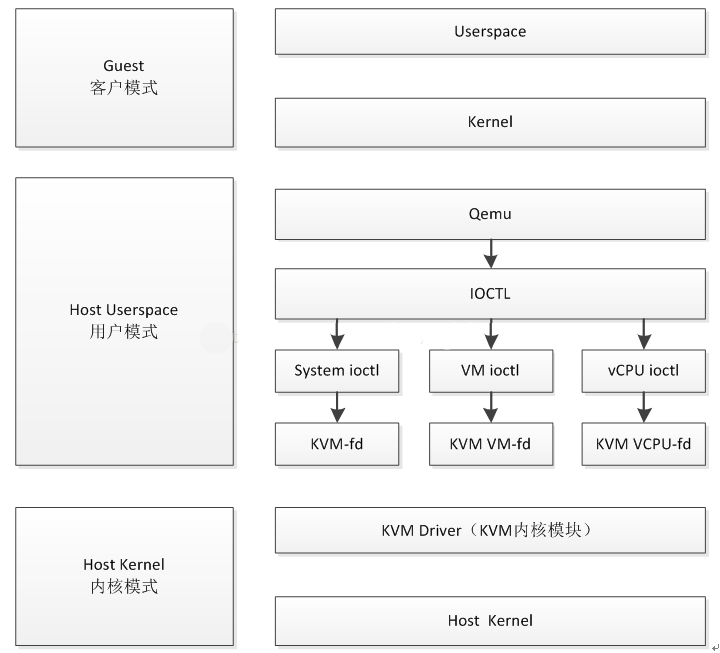
\includegraphics[width=0.6 \textwidth]{figs/KVM三种模式的层次关系.png}
  \caption{KVM三种模式的层次关系}
  \label{fig:kvm} %设置图形引用名称
\end{figure}
%『h』当前位置。将图形放置在正文文本中给出该图形环境的地方。如果本页所剩的页面不够,这一参数将不起作用。
%『t』顶部。将图形放置在页面的顶部。
%『b』底部。将图形放置在页面的底部。
%『p』浮动页。将图形放置在一只允许有浮动对象的页面上。
